\section{Skin-Deep Identities}

\textit{14 December 2016}

In contemporary times, indigenous identities exist in a delicate state.  They
are defined in part by political boundaries, enforced by cultural expectations,
and developed in an on-going relationship with the dominant, colonizing culture.
With all of these factors in place, the self-determination of what remains
essential for indigenous identities falls to how an individual chooses to
present themselves; the visible aspects of their culture become a way to control
and dictate their identity. Subsequently, the discourse around the artistic
practices of an indigenous group provides an opportunity to negotiate the
boundaries of identity. This appears most saliently when examining issues
surrounding tattoos; such a living, physical process allows individuals to
demonstrate an indelible part of themselves, while challenging the lines between
cultures and extending traditional practices into the present.

Contemporary tattoo culture grew from a mottled history. European explorers of
the 18th century who encountered tattooed natives associated the appearance and
practice with primitive, savage barbarism; in the modern Euro-American society,
tattoos are often associated with ``alternative'' subcultures, criminals,
bikers, sailors, and other rough characters. It persists as a representative of
a marginalized class in either case. At the same time, tattoos hold important
cultural histories and spiritual significance for indigenous groups, and provide
a vehicle for modern people to explore their own identities. These different
perspectives on tattoo creates a line of friction, along which some exchanges
take place that raise further questions about how identities are defined.

Traditional tattoo practice as a coming of age ritual in Polynesian groups
demonstrated the completion of a series of ordeals, the purpose of which
Nicholas Thomas describes are ``understood to harden the body...while signifying
maturity of a particular phase of adolescence'' \footnote{Thomas, 102}. This
ritual of pain creates a connection that comes from a shared experience;
specific motifs used in a particular tattoo serves as a permanent visible mark
to make a variety of statements about the individual. In more traditional uses,
this includes elaborate visual armor to signify a powerful
warrior\footnote{ibid., 104}, marks for desanctifying the body as a sign of
growth\footnote{ibid., 108}, and, consequently, the bestowing of a status and
rank on the tattooed that contributed to their social power\footnote{ibid.,
103}. In more general terms, tattoos are a specific form of communication, which
demonstrate cultural affiliations and belief systems. In other words, they are a
critical aspect of the identity of tattooed people, allowing them to forge a
connection between their bodies and their identities, as well as signal this
identity to others.

In a modern setting, Polynesian tattooing practices retained its ties to
traditional roots in spite of colonial efforts to eradicate it. This was a
controversial issue, especially regarding the appearance and social roles of
Maori women who wore \textit{moko} (traditional Maori tattoos); Ngahuia Te
Awekotuku credits it specifically as ``an enhancement of Maori women's beauty on
Maori terms, and it both repelled and fascinated the European
viewer.''\footnote{Te Awekotuku, pp. 85} As a highly visible mark that
represented a core part of the Maori power structure and cosmology,
\textit{moko} directly challenged what Europeans deemed desirable, and what
Christians deemed permissible. Owing to the persistence of tattoo practice,
\textit{moko} survived colonization, and thus did the Maori people who carried
it through.

This continuity of culture can be seen in Te Awekotuku's profiles of modern
Maori women; photographs and memories of elder women with \textit{kauae}
(distinct facial tattoos of intricate linework around the chin and lips) play a
significant role in the image of themselves that those women choose to present
to the world. By wearing \textit{moko} that alludes to their elders, these women
maintain a social continuity that draws their pasts into the present. She also
observes that ``most meditate on desire and beauty'' and that ``transforming the
body, transforming the face was primarily about pleasing one's
self''\footnote{ibid., 90}, an approach which highlights choosing \textit{moko}
as a deliberate act of self-determination; these women prioritize what the
\textit{moko} signifies for their own identities and histories, and other
aspects---such as the circumstances around their tattooing, and how they are
perceived by non-Maori---become secondary.

As the primary function of \textit{moko} then  becomes an act for women to
visually display their own identities, some of the ties with traditional tools
and practice fall in importance. Combined with the prevalence of modern electric
tattooing machines, this has led to \textit{moko} application by non-Maori,
using modern technology. Te Awekotuku includes a personal story from Roger
Ingerton, a non-native tattoo artist in Wellington, New Zealand. When he was
first approached for a \textit{moko} by a Maori woman, he was the only tattoo
artist in the area. Even though he had never applied a traditional facial
tattoo, he was asked to do so, and many other Maori women followed that first
one\footnote{ibid., 91}; this illustrates that the act of wearing that identity
eclipsed the connection to the traditional practice from which those visuals
originated.

In this instance, the process of the tattoo begins from a negotiation between an
indigenous person with a cultural background that gives her the desire and
rights to wear a particular design, and a non-indigenous person who has the
skills and tools to actualize that desire. This negotiation includes selecting
motifs, determining proper placement, and agreeing on a price, all of which is
complicated by introducing someone who does not share the identity of the
tattooed. For Ingerton, this process was clearly a difficult one; he sought
advice from a local Maori elder when felt he lacked the background to work on
\textit{moko}, and described tattooing as ``like diamond cutting, and a person
is a million-dollar diamond''\footnote{ibid}. He eventually stepped back from
facial tattoos, recommending that subsequent inquirers seek practitioners within
their own tribes as a more appropriate exchange.

This relationship is almost reversed in some of the blending of modern Native
American tattoo practice. Maureen Schwartz consulted with a variety of tattooed
and tattooists, all of whom have some aspects of Native American motifs in their
tattoos. She draws a relationship between those tattoos and a desire for the
``primitive'', which ``demonstrate that notions of Indians or Indianness
continue to play a vital role in contemporary American notions of
identity''\footnote{Schwartz, 225}. Her study of Richard Cioppa's approach to
getting tattoos keenly illustrates this process; he started collecting tattoos
of wolf imagery because he felt a connection with wolves after living on the
streets\footnote{ibid., 227}, but he also used the image of a Native American
man in a wolf skin\footnote{ibid., 232}. Through using tattoos to help define
himself after getting off the streets, Schwartz claims that ``[t]attoos etch
identity onto the body, they simultaneously erase what is already there: in many
cases, what is eradicated is one's whiteness''\footnote{ibid., 228}. Cioppa, by
Schwartz's view, is replacing a part of his identity tied to his ethnicity with
an identity he built by combining his life experiences with his perception of
the symbolism in indigenous imagery.

\begin{figure}[ht!]
  \centering
  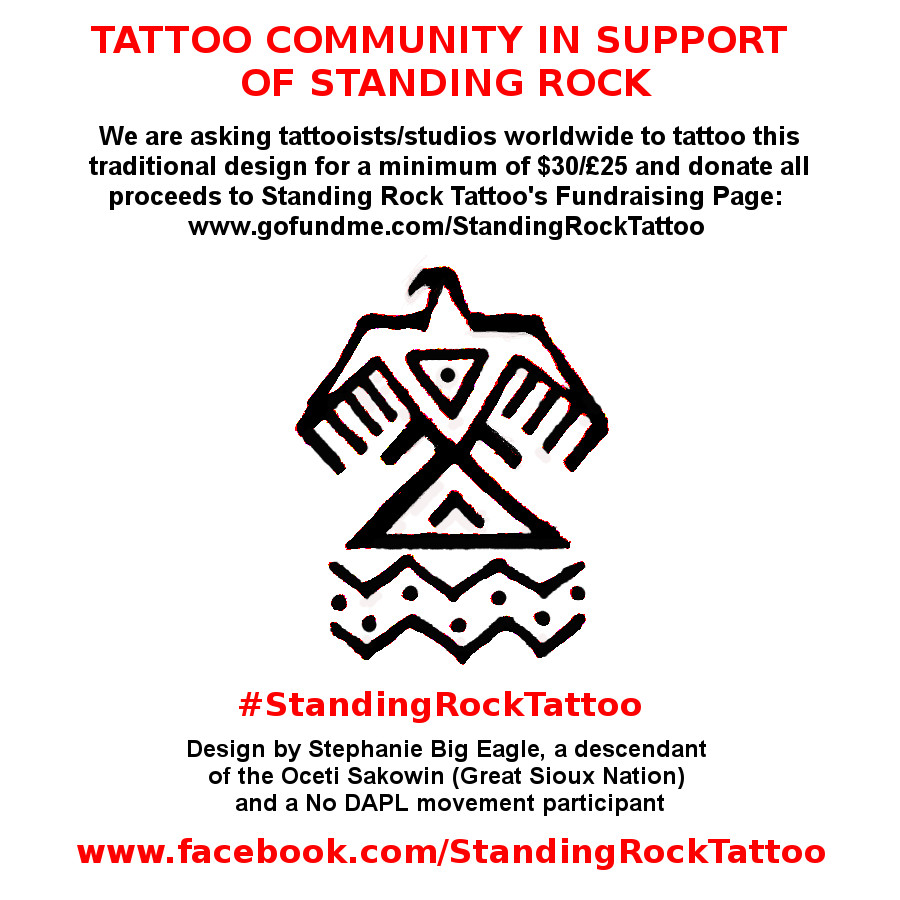
\includegraphics[width=90mm]{standingrock.jpg}
  \caption{Standing Rock Tattoo Flyer\label{overflow}}
\end{figure}

In 2016, tattoo artist Stephanie Big Eagle (Dakota/Sioux) released a tattoo
design to raise funds and solidarity in support of camps involved with the No
Dakota Access Pipeline (NoDAPL) movement at the Standing Rock Sioux Reservation;
a flyer that included donation instructions and the original design circulated
on social media (fig. 1). From her description of the design, Stephanie Big
Eagle emphasizes its role as a symbol of native people standing against a
colonizing force; its central figure is a thunderbird, representing the Sioux
life-giver and protection spirit, with a circle in its heart to stand for the
unity of the wide range of tribal representation within the NoDAPL movement.
Instructions from the artist released permission for the design to be worn by
``anyone'', so long as a minimum donation of \$30 was made to the campaign.  The
design raised over \$100k within its first month\footnote{\textit{GoFundMe}, as
of 12 December 2016}; a registry of participating tattoo studios includes over a
hundred entries from around the world.

The creation of a tattoo design for a specific event is not unique to this
instance, but in this case, the unity of native and non-native tattooist and
tattooed demonstrates a blurring of identity lines that challenges existing
norms about who owns indigenous art. A news article from Shreveport, Louisiana,
interviewed a variety of residents who, despite both a cultural and physical
distance from the Standing Rock Sioux tribe, decided to receive Big Eagle's
design from a local tattoo artist with no native affiliations \footnote{Talamo}.
Reasons given by those who chose the tattoo ranged from reconnecting with tribal
history, outwardly displaying support for Native American rights, and signifying
personal changes from participating in the NoDAPL movement. For many people,
this was their first tattoo, as their association with the NoDAPL movement
significantly affected their worldviews; this acceptance of the image on their
skin resonates with the Maori usage of \textit{moko} as a permanent, external
representation of a profound personal change.

Tattoos exist at the border between a body and the rest of the world. Their
visual nature communicates something about the wearer to the viewer, whether
that viewer is a member of their tribe or not. In a modern, global setting,
images of specific tattoos and motifs circulate rapidly; tattoos quickly become
part of larger statements of identity, alignment, and self. For some groups,
like the Maori women, tattoo occupies a critical element of self-definition,
which includes the outward display of their personal imagery. For others, like
Robert Cioppa, using indigenous motifs in his tattoos allowed him to create an
identity that he felt proud of, by replacing parts of himself he'd grown past.
On a larger scale, like those who took part in the mass acquisition of the
Standing Rock Tattoo, indigenous tattoos become a vehicle for making a political
statement, while marking a permanently visible commitment to a cause. The border
tattoos create is only skin-deep, but that enables a constantly shifting field
on which identities are drawn.
